\documentclass[12pt,a4paper]{instrumentacao}

\usepackage{listings}

\graphicspath{
	{../Resources/Images/}
	{../Resources/Mathematica/images/}
}

\title{Central meteorológica: Dispositivo para medição de precipitação, de temperatura e de velocidade do vento}
\author{Rogiel Sulzbach \and Rodrigo de Castro Silveira}
\startdate{18 de abril de 2016}
\finishdate{27 de junho de 2016}
\emails{
	\emailaddress{R.J.S.}{rogiel@rogiel.com} e
	\emailaddress{R.C.S.}{csilveira.rodrigo@gmail.com}
}
\resume{Este trabalho visa o desenvolvimento do trabalho final da disciplina cujo objetivo é construir uma estação meteorológica que permite fazer algumas medições que, através dos dados recolhidos em um determinado período, contribuem para fazer a previsão de tempo e também a caracterização do clima. Para tanto, será desenvolvido instrumentos (ou sensores eletrônicos) de medição que registram as variáveis meteorológicas e climáticas. Como uma estação meteorológica possui muitos instrumentos de medição, para este trabalho, serão feitos apenas alguns deles, tais como o termômetro para medir a temperatura, o anemômetro para medir a velocidade do vento e o pluviômetro para medir a precipitação pluviométrica}
\abstract{This class final project objective is to build a meteorological station which allows to collect data over time whose measurements contribute to weather and to climate characterization. For such, sensors and electronic sensors will be developed which will register meteorological variables. As a meteorological station has several instruments, only a subset of those will be implemented on this project, these include a thermometer to measure temperatures, anemometer to measure the wind speed and a rain gauge to measure the rainfall.}
\keywords{estação meteorológica; instrumentos de medição; temperatura; quantidade de chuva; velocidade de vento.}
\institute{Universidade Federal do Rio Grande do Sul, Departamento de Engenharia Elétrica, Curso de Engenharia Elétrica, Instrumentação A, Prof. Dr. Alexandre Balbinot}

\headertext{Anteprojeto}

\begin{document}
\maketitle

\chapter{Introdução}
De acordo com o livro-texto da disciplina \textit{ENG04457 - Instrumentação A} \cite{livro-texto}, em seu prefácio, expõe que "hoje o mundo não escreve: digita. Internet, iPod, celulares, pen-drives... Toda essa revolução na sociedade criou novas habilitações dentro das engenharias, como, por exemplo, as engenharias de computação, de software e de tecnologia da informação. O analógico aparentemente tornou-se obsoleto, tirando a atenção de disciplinas relacionadas, como instrumentação, sensores e transdutores -- um equívoco ocorrido em função da compreensão superficial do que está por trás desta revolução tecnológica que estamos vivendo. Porém, o som, a imagem e diversos outros fenômenos que nos cercam são entes analógicos. Antes de virar bytes, o mundo é captado analogicamente". É com base nesta necessidade do domínio da captação do mundo analógico que a disciplina corretamente propõe a elaboração, planejamento e montagem de um projeto experimental utilizando os conceitos vistos em sala de aula.

O grupo, orientado por algumas indicações do professor da disciplina, optou pela elaboração do projeto de uma \textit{Central Meteorológica} capaz de executar medições de precipitação (chuva), de temperatura e de velocidade do vento. De acordo com a enciclopédia eletrônica livre \textit{Wikipedia}\cite{estacao}, "uma estação meteorológica é um local onde são recolhidos dados para análise do tempo meteorológico. Encontram-se equipadas com instrumentos (ou sensores eletrônicos) de medição e registro das variáveis meteorológicas/climáticas. Os seus dados são utilizados para a previsão do tempo e para a caracterização do clima, pelo que também podem ser designadas por estações climatológicas".

O projeto desenvolvido pelo grupo fará a captação e tratamento dos dados de temperatura, velocidade do vento e volume de precipitação. Assim, serão projetados os seguintes instrumentos:

\begin{itemize}
	\item \textbf{Termômetro}: para medir a temperatura;
	\item \textbf{Anemômetro}: para medir a velocidade do vento;
	\item \textbf{Pluviômetro}: para medir a precipitação pluviométrica.
\end{itemize}

\chapter{Metodologia Experimental}
A seguir serão apresentadas as especificações de cada um dos instrumentos que estão sendo projetados e implementados para a montagem da Central Meteorológica, objeto do projeto final da disciplina.

\section{Termômetro}
Para a implementação do termômetro será utilizado um sensor do tipo RTD (\textit{Resistance Temperature Detectors}) a fim de medir a temperatura do ar ambiente onde a estação está instalada. A faixa de medição de interesse foi estipulada de $-10ºC$ a $+50ºC$, e será tentado uma resolução de $0.1ºC$. Os termômetros de resistência funcionam com base no fato de que, de modo geral, a resistência dos metais aumenta com a temperatura \cite{livro-texto}. As principais características dos RTDs são:

\begin{itemize}
	\item Condutor metálico (a platina é o metal mais utilizado);
	\item São dispositivos praticamente lineares;
	\item Dependendo do metal são muito estáveis;
	\item Apresentam baixíssima tolerância de fabricação (0,06\% a 0,15\%).
\end{itemize}

O RTD utilizado será um Pt100, que é um RTD de platina que apresenta $100\Omega$ @ $0ºC$. O modelo utilizado é o DM-301, da LABFACILITY. Segundo catálogo \cite{catalogo-pt100} disponibilizado por um distribuidor do sensor, o DM-301 é um sensor Pt100 do tipo película fina, para uso de $-50ºC$ a $+500ºC$, classe B da norma IEC751. Sua resistência no ponto de fusão da água ($0ºC$) é de $100\Omega$, apresenta um intervalo fundamental ($0ºC$ a $100ºC$) de $38.5\Omega$ (nominal), resposta térmica de $0.1s$ e estabilidade $\pm 0.05\%$. A Figura \ref{fig:DM-301} apresenta uma foto do sensor DM-301. Já a Figura \ref{fig:termometro-ilustracao} apresenta a ilustração com a montagem do sensor em uma estrutura para utilização no experimento.

\begin{figure}[H]
	\centering 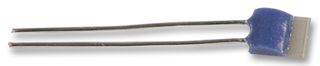
\includegraphics[width=0.5\textwidth]{DM-301.jpg}
	\caption{Foto do sensor resistivo Pt100, modelo DM-301, da LABFACILITY.}
	Fonte: \url{https://www.digchip.com/datasheets/parts/datasheet/2403/DM-301.php}
	\label{fig:DM-301}
\end{figure}

\begin{figure}[H]
	\centering 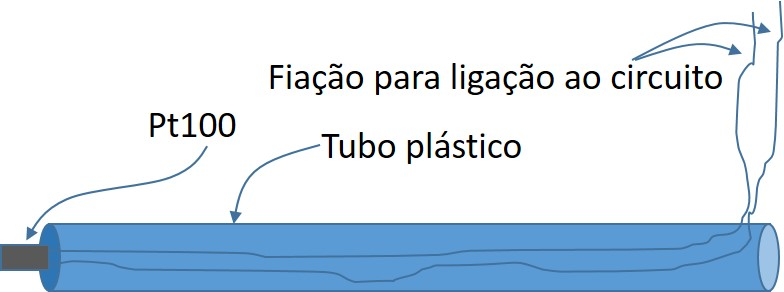
\includegraphics[width=0.5\textwidth]{termometro-ilustracao.jpg}
	\caption{Ilustração com a montagem do sensor Pt100 em uma estrutura para utilização no experimento.}

	\label{fig:termometro-ilustracao}
\end{figure}

A classe B de tolerância, segundo a norma IEC751, apresenta um coeficiente térmico $\alpha = 0.003850 \Omega/\OmegaºC \pm 0.000063$, e um $R_0= 100\Omega \pm 0.12\%$. Os desvios admissíveis, para temperatura e resistência, são observados nas Equações \ref{eq:pt100-desvio-admissivel-temp} e \ref{eq:pt100-desvio-admissivel-resist}, respectivamente.

\begin{equation}
	T(ºC)=\pm (0.3+0.005*t)
	\label{eq:pt100-desvio-admissivel-temp}
\end{equation}
\begin{equation}
	R(\Omega)=\pm (0.12+0.0018*t)
	\label{eq:pt100-desvio-admissivel-resist}
\end{equation}

Usando-se os valores-padrão estabelecidos pela norma IEC751 para sensores Pt100, pode-se chegar à função de transferência teórica aproximada para esse sensor:

\begin{equation}
	R=R_0(1+\alpha(T-T_0))
	\label{eq:pt100-eq-teorica}
\end{equation}

\noindent onde $R_0$ é a resistência elétrica na temperatura $T_0$ e $\alpha$ é o coeficiente térmico da platina. Substituindo-se os valores na Equação \ref{eq:pt100-eq-teorica}, tem-se:

\begin{equation}
	R=100+0.385*T
	\label{eq:pt100-eq-teorica-valor}
\end{equation}

Tendo a sensibilidade teórica desse sistema representado por:

\begin{equation}
	S=0.385 [\Omega/ºC]
	\label{eq:pt100-sensibilidade-teorica-valor}
\end{equation}

Um típico condicionamento dado a RTDs utiliza o método baseado em uma ponte de Wheatstone. A Figura \ref{fig:termometro-ponte} apresenta o esquemático da estrutura básica da Ponte utilizada.

\begin{figure}[H]
	\centering 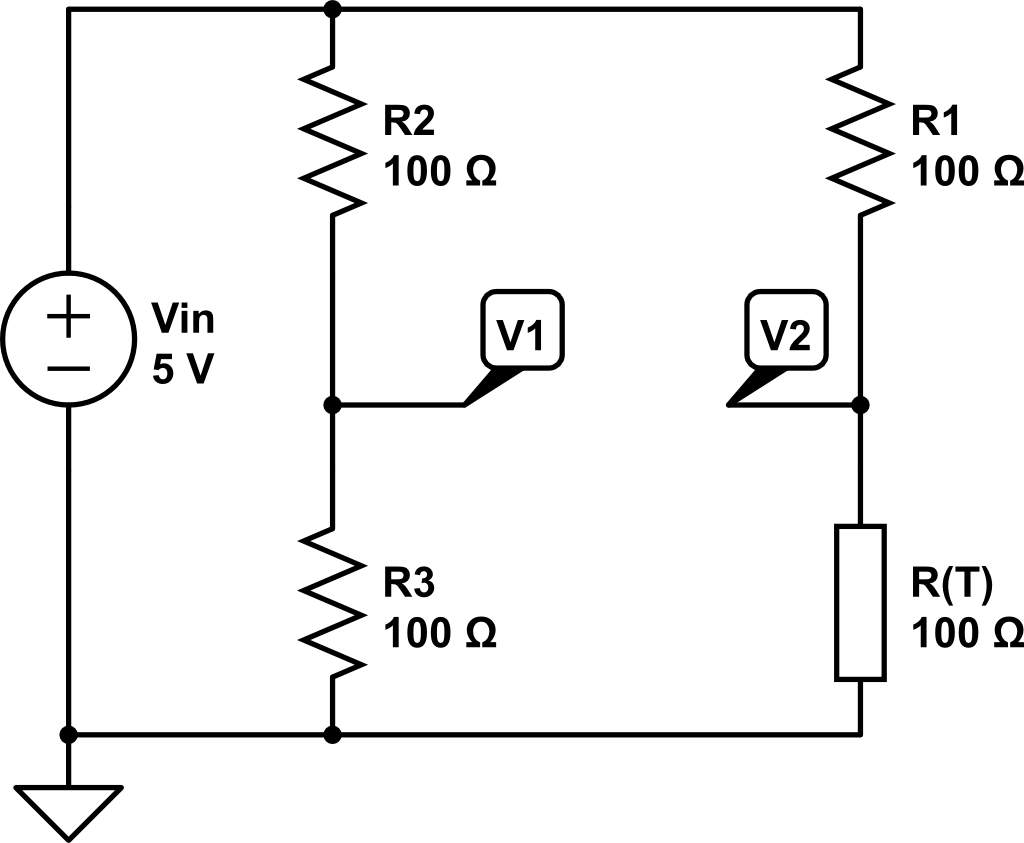
\includegraphics[width=0.5\textwidth]{pt100-ponte.png}
	\caption{Esquemático da estrutura básica da ponte de Wheatstone utilizada como parte do circuito condicionador do Pt100.}
	\label{fig:termometro-ponte}
\end{figure}

\noindent onde $R_1=R_2=R_3$ são resistores de $100\Omega$ e $R(T)$ é o sensor Pt100 com $100\Omega@0ºC$. $V_{in}$ é uma fonte de tensão de $5V$, e $V_1$ e $V_2$ são os nós diferenciais da ponte.

Equacionando o circuito apresentado na Figura \ref{fig:termometro-ponte}, para a saída diferencial, tem-se:

\begin{equation}
	V_{out}=V_1-V_2=\frac{R_2R(T)-R_3R_1}{(R_2+R_3)(R_1R(T))}V_{in}
	\label{eq:termometro-ponte-saida}
\end{equation}

Substituindo-se, na Equação \ref{eq:termometro-ponte-saida}, pelos valores nominais dos resistores, tem-se:

\begin{equation}
	V_{out}=2.5-\frac{500}{R(T)+100}
	\label{eq:termometro-ponte-saida-valores}
\end{equation}

A ponte de Wheatstone tem como característica principal o atingimento da tensão diferencial igual a zero para a seguinte relação:

 \begin{equation}
	R_1*R_3=R_2*R(T)
	\label{eq:termometro-ponte-equilibrio}
\end{equation}

Para os valores indicados, a situação explicitada na Equação \ref{eq:termometro-ponte-equilibrio} só acontece para $R(T)=100\Omega$, isto é, quando o sensor estiver percebendo uma temperatura de $0ºC$. Neste caso, a tensão diferencial é de $0V$.

Porém, como a temperatura mínima a ser medida é de $-10ºC$, é interessante que se tenha um circuito para o ajuste de \textit{offset}, na qual se consiga ajustar o valor de   saída em $0V$, independente do valor de $R(T)$. Para isso, será implementado um circuito divisor de tensão, com um potenciômetro alimentado com tensão simétrica e um resistor em série com o cursor do potenciômetro, ligado ao nó $V_1$ da ponte, conforme pode ser verificado na Figura \ref{fig:termometro-ponte-offset}.

\begin{figure}[H]
	\centering 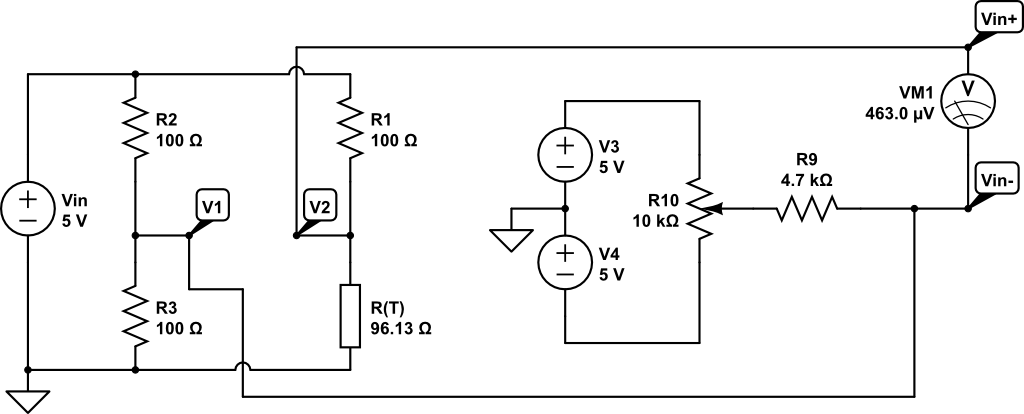
\includegraphics[width=\textwidth]{pt100-ponte-offset.png}
	\caption{Esquemático da estrutura básica da ponte de Wheatstone e um circuito para correção de offset utilizada como parte do circuito condicionador do Pt100.}
	\label{fig:termometro-ponte-offset}
\end{figure}

Associado ao circuito da ponte de Wheatstone e ao circuito de correção de offset, deve-se utilizar um amplificador de instrumentação (AI), a fim de deixar os níveis de tensão de saída mais apropriados ao nível de tensão de entrada do ADC. Para isto, será utilizado o AI INA126 \cite{datasheet-INA126}, da Texas Instruments. Esse AI possui um ganho expresso por:

 \begin{equation}
	G=5+\frac{80k\Omega}{R_G}
	\label{eq:ganho-INA126}
\end{equation}

\noindent onde $R_G$ é um resistor conectado aos pinos 1 e 8 do CI, em função do ganho escolhido.

A Figura \ref{fig:termometro-ckt-condicionador-completo} mostra o circuito condicionador proposto para o Pt100, com a ponte de Wheatstone, o circuito corretor de offset e o AI INA126.

\begin{figure}[H]
	\centering 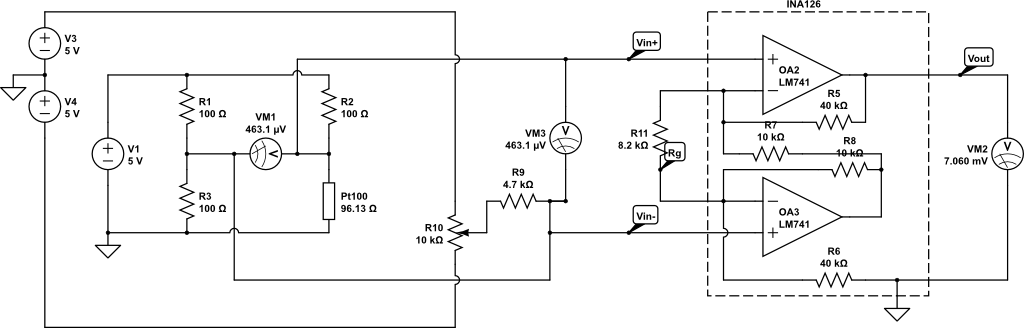
\includegraphics[width=\textwidth]{pt100-ponte-com-ina-min.png}
	\caption{Esquemático da estrutura básica de condicionamento proposto para o Pt100.}
	\label{fig:termometro-ckt-condicionador-completo}
\end{figure}

Com base na estrutura de condicionamento proposta e os valores teóricos da função de transferência do Pt100 (Equação \ref{eq:pt100-eq-teorica-valor}), pode-se elaborar a Cadeia de Medidas proposta para o termômetro a ser implementado, verificada na Figura \ref{fig:termometro-cadeia-medidas-proposta}.

\begin{figure}[H]
	\centering 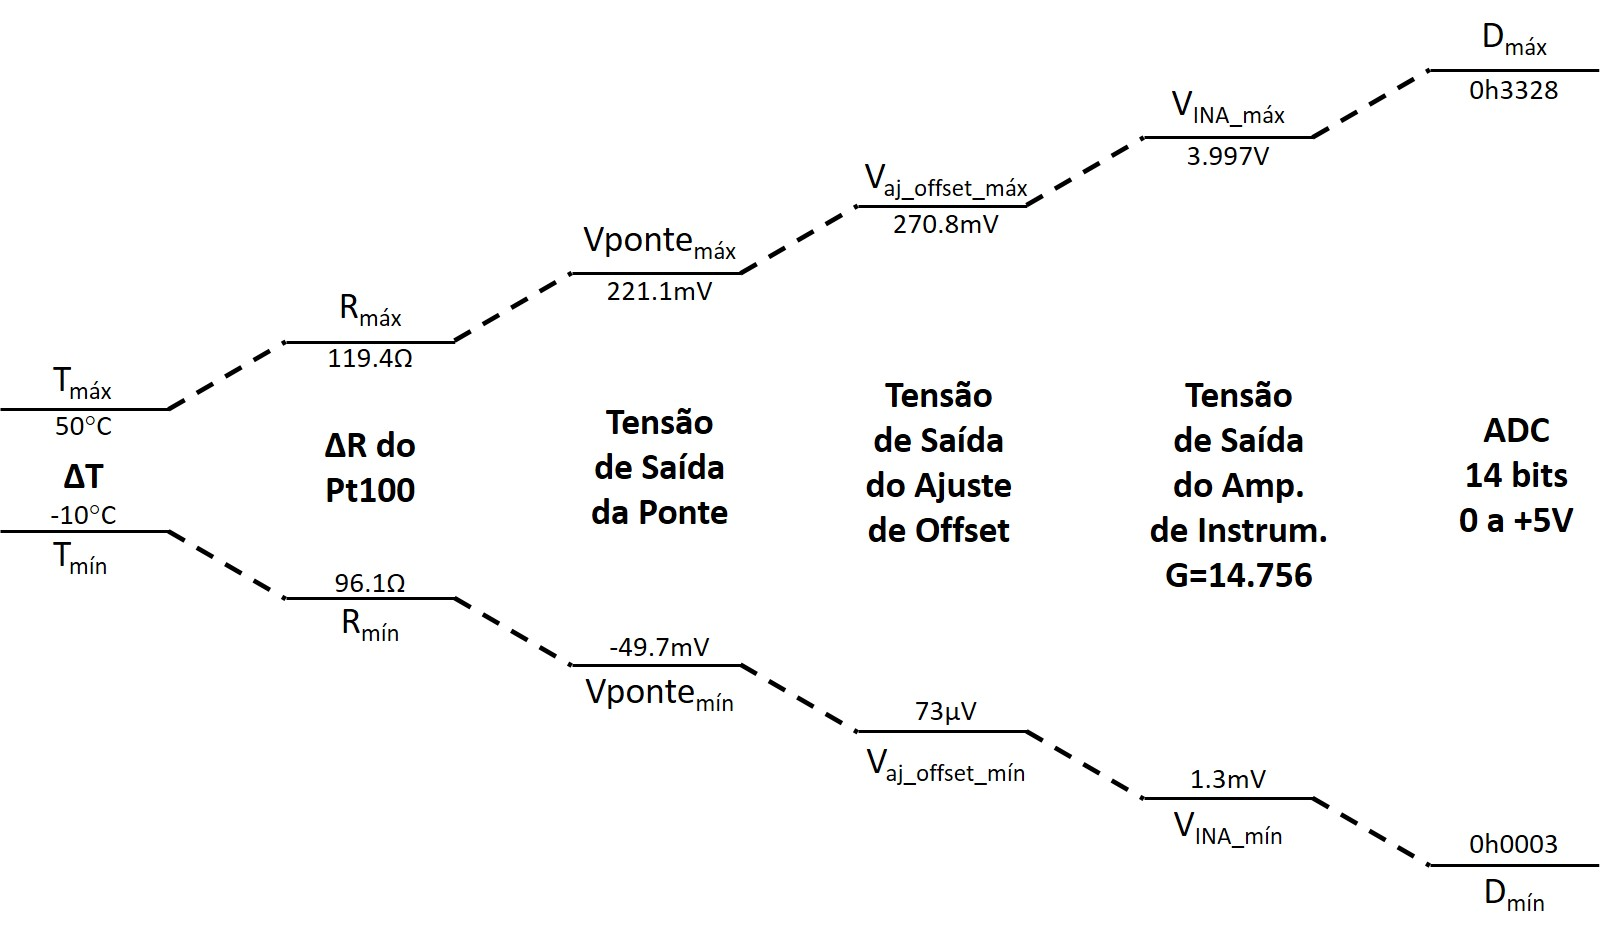
\includegraphics[width=\textwidth]{termometro-cadeia-medidas-proposta.jpg}
	\caption{Cadeia de Medidas proposta para o termômetro a ser implementado.}
	\label{fig:termometro-cadeia-medidas-proposta}
\end{figure}

\section{Anemômetro}
O anemômetro é um instrumento que mede a velocidade do vento horizontal. Os anemômetros de copo são o tipo padrão de anemômetro, pois são robustos e resistentes aos ventos oblíquos causados por mastros e travessas, e este tipo será utilizado no projeto em questão, a exemplo da Figura \ref{fig:anemometro}

\begin{figure}[h]
	\centering
		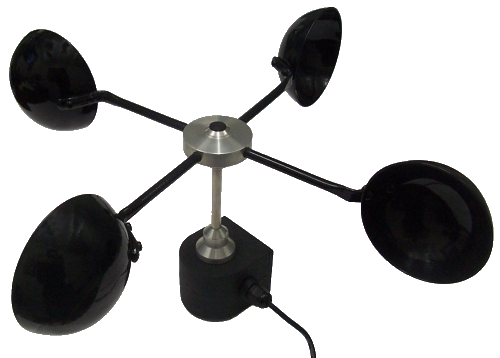
\includegraphics{Figuras/anemometro.png}
	\caption{Exemplo de anemômetro de copo}
	Fonte: \url{https://www.google.com.br/url?sa=i&rct=j&q=&esrc=s&source=images&cd=&cad=rja&uact=8&ved=&url=http\%3A\%2F\%2Fwww.seinstrumentos.com.br\%2Fanemometro.html&psig=AFQjCNGjijn5ng5hpmUAcBq4F_TVvceWUw&ust=1461032511805601}
	\label{fig:anemometro}
\end{figure}

Como forma de medir a velocidade de rotação do anemômetro, será utilizado um sensor de efeito \textit{Hall} associado com um ímã. Assim, toda vez que o ímã passar pelo sensor de efeito \textit{Hall}, este deixa passar corrente, podendo assim ser contabilizado o número de voltas em um determinado período de análise.


\section{Pluviômetro}
Segundo a Wikipedia \cite{pluviometro}, "o pluviômetro é um aparelho de meteorologia usado para recolher e medir, em milímetros lineares, a quantidade de líquidos ou sólidos (chuva, neve, granizo) precipitados durante um determinado tempo e local". O parâmetro determinado por esse instrumento chama-se \textit{índice pluviométrico}, que é o somatório da precipitação num determinado local durante um período de tempo estabelecido, medido em milímetros [$mm$]. Como o equipamento mensura a quantidade de chuva que precipita, é elementar para estudos meteorológicos e hidrológicos em conjunto com o sensor de temperatura.

A estrutura física do pluviômetro consiste em um sistema de captação de chuva, com uma área determinada, e um reservatório para coleta do material captado. Nesse reservatório há um sensor que possibilita medir a diferença do nível de fluído armazenado.

Como o equipamento mensura a quantidade de chuva que precipita, é elementar para estudos meteorológicos e hidrológicos em conjunto com o sensor de temperatura. Um dos princípios de funcionamento composto é feito por um sensor de precipitação tipo báscula, um equipamento que mensura a massa de um corpo, pois o índice pluviométrico em milímetros indica o volume em litros de água que caíram em um metro quadrado de área, assim uma chuva de 20 mm corresponderá à precipitação de 20 litros de água por metro quadrado, logicamente sempre na horizontal. Como quaisquer equipamentos automáticos, um software de coleta e tratamento de dados é utilizado para relatórios temporais e análises das características da chuva. Como a maneira de medir a quantidade de chuva é muito ampla, cabe os membros do grupo investigar o melhor tipo de sensor e metodologia de medição apropriados para obter boas medidas. 

Optou-se por utilizar um sensor capacitivo com referência baseada em um documento do "TI Designs"\cite{pluviometro-capacitivo-texas} onde é proposto um sensor simples de medida de capacitância utilizando uma placa de circuito impresso com duas placas paralelas. A fim de determinar a validade do \textit{design} de sensor, foi confeccionado um sistema simples com uma placa de circuito impresso contendo duas barras que funcionam como eletrodos do sensor e a placa foi fixada na face interna de um recipiente e acrílico. A placa foi isolada com verniz para evitar que a água fizesse contato elétrico entre os eletrodos. O recipiente possui dimensões internas de 3cm por 6cm com 15cm de altura e foi confeccionado sob medida.

A Figura \ref{fig:sensor-nivel-capacitivo} apresenta um desenho esquemático do sensor de nível

\begin{figure}[H]
	\centering 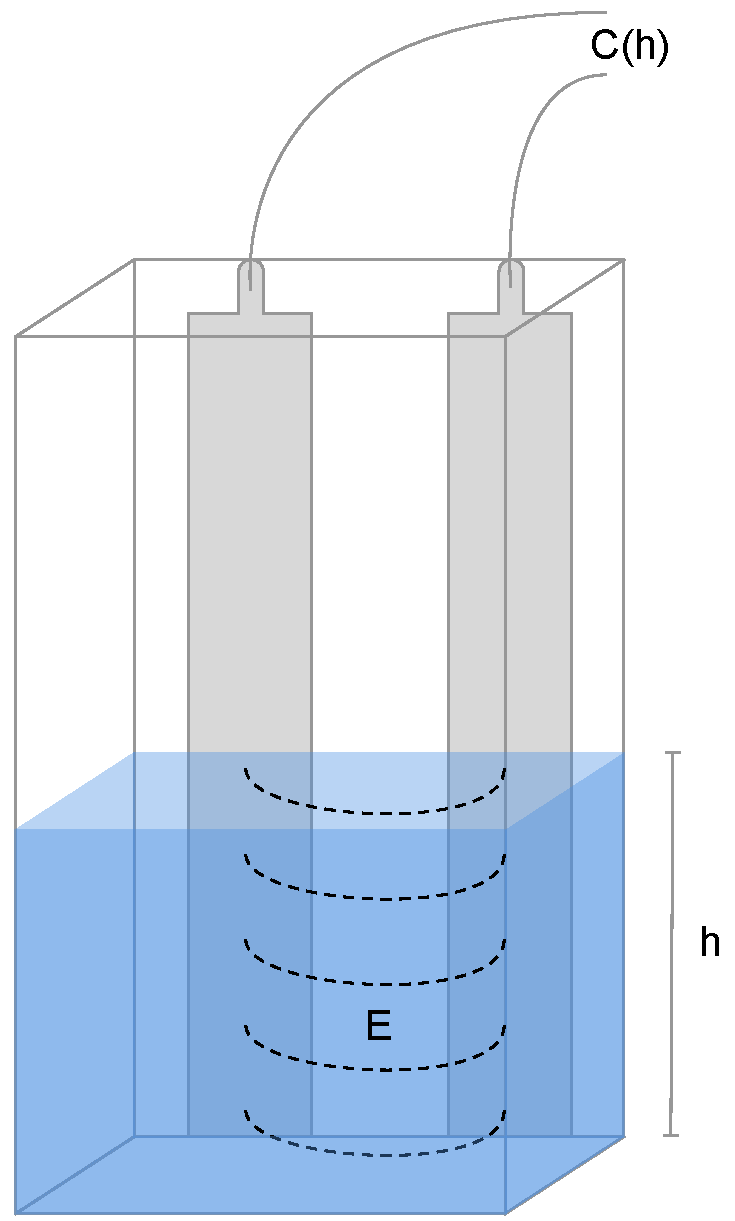
\includegraphics[width=0.5\textwidth]{SensorNivelCapacitivo.pdf}
	\caption{Desenho esquemático do sensor de nível capacitivo. $C(H)$ é a capacitância equivalente da construção para um nível de água $h$ e $E$ são as linhas de campo elétrico internas no sensor.}
	\label{fig:sensor-nivel-capacitivo}
\end{figure}

A fim de determinar a viabilidade de medição deste sistema, um experimento rápido foi realizado onde a função de transferência da capacitância do sistema foi extraída utilizando um multímetro Minipa ET-2082B \cite{multimetro-minipa} na escala de 20nF e 200 nF (onde aplicável) para a medição da capacitância para volumes de água entre 0 mL e 200 mL com resolução de 2mL.

O condicionamento do sensor ainda não foi testado, mas acredita-se que a melhor topologia para esta aplicação consiste em um amplificador numa topologia de integrador conectado a um comparador que compara a curva de carregamento do capacitor com uma referência fixa. A variação de frequência do sistema corresponde à variação de capacitância, que incorre em uma variação de frequência de oscilação do sistema. A Figura \ref{fig:sensor-nivel-capacitivo-condicionamento} apresenta o circuito de condicionamento.

\begin{figure}[H]
	\centering 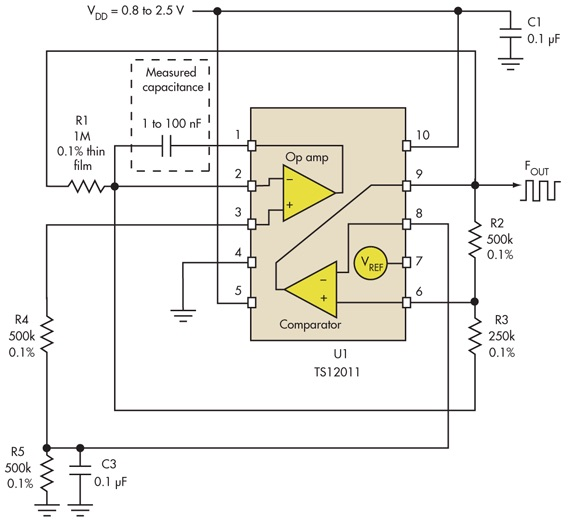
\includegraphics[width=\textwidth]{SensorNivelCapacitivo-Condicionamento.jpg}
	\caption{Desenho esquemático do sensor de nível capacitivo. $C(H)$ é a capacitância equivalente da construção para um nível de água $h$ e $E$ são as linhas de campo elétrico internas no sensor.}
	Fonte: Electronic Design \cite{medicao-capacitancia}
	\label{fig:sensor-nivel-capacitivo-condicionamento}
\end{figure}

\chapter{Resultados e discussões}

\section{Termômetro}

Com base nas especificações do sensor Pt100 já estabelecidas, efetuou-se uma verificação do seu funcionamento, analisando-se a variação da sua resistência elétrica em função da variação de temperatura. O experimento realizado retornou os resultados que podem ser observados na Tabela \ref{tab:pt100-resistencia-exp}.

\begin{table}[H]
\centering
\caption{Valores experimentais da variação da resistência elétrica do sensor Pt100 em função da variação da temperatura}
\label{tab:pt100-resistencia-exp}
\begin{tabular}{|c|c|}
\hline
\textbf{$T(ºC)$} & \textbf{$R(T)(\Omega)$} \\ \hline
11.3           & 104.4                       \\ \hline
13.3           & 105.3                       \\ \hline
15.8           & 106.2                       \\ \hline
18.5           & 107.3                       \\ \hline
20.9           & 108.2                       \\ \hline
23.4           & 109.2                       \\ \hline
25.9           & 110.1                       \\ \hline
27.7           & 110.8                       \\ \hline
29.7           & 111.5                       \\ \hline
31.6           & 112.2                       \\ \hline
33.8           & 113.2                       \\ \hline
35.6           & 113.8                       \\ \hline
38.7           & 115.0                       \\ \hline
41.1           & 115.8                       \\ \hline
42.7           & 116.4                       \\ \hline
45.2           & 117.2                       \\ \hline
49.3           & 118.9                       \\ \hline
50.3           & 119.4                       \\ \hline
\end{tabular}
\end{table}

Na Figura \ref{fig:pt100-tf-experimental} é possível verificar o gráfico com os valores adquiridos e apresentados na Tabela \ref{tab:pt100-resistencia-exp} (pontos), bem como o traçado da função de transferência levantada por regressão linear (linha contínua), com base nos dados obtidos experimentalmente.

\begin{figure}[H]
	\centering 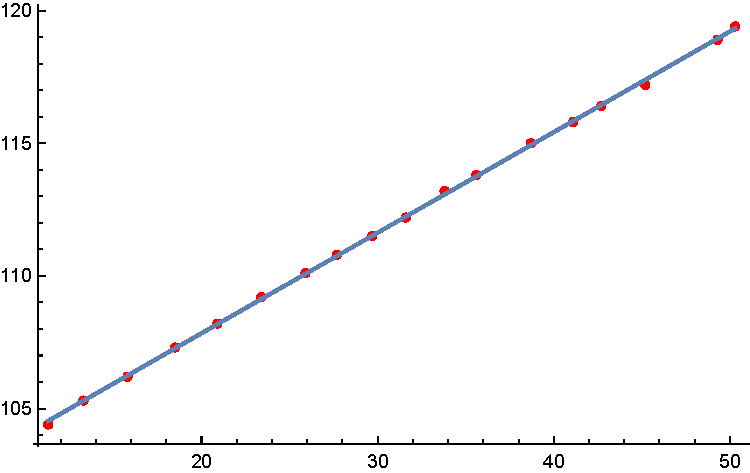
\includegraphics[width=\textwidth]{Temperatura/ResistenceTransferFunction.pdf}
	\caption{Amostra dos valores de resistência obtidos pela variação da temperatura do Pt100 e função de transferência experimental.}
	\label{fig:pt100-tf-experimental}
\end{figure}

A Equação \ref{eq:pt100-tf-experimental} apresenta a função de transferência experimental, levantada com base na regressão linear utilizando-se os valores constatados experimentalmente.

\begin{equation}
	R(T)=100.25+0.3792T
	\label{eq:pt100-tf-experimental}
\end{equation}

Apresentando um valor de $R^2$ de:

\begin{equation}
	R^2=0.9997
	\label{eq:pt100-r2-tf-experimental}
\end{equation}

Com base na função de transferência experimental apresentada na Equação \ref{eq:pt100-tf-experimental} é possível encontrar a sensibilidade experimental $S_{exp}$ do sistema, bem como o coeficiente de temperatura experimental $\alpha_{exp}$ do Pt100 utilizado.

\begin{equation}
	S_{exp}=\frac{dR(T)}{dT}=0.3792\frac{\Omega}{ºC}
	\label{eq:pt100-sensibilidade-experimental}
\end{equation}

\begin{equation}
	\alpha_{exp}=0.003783\Omega/\OmegaºC
	\label{eq:pt100-alpha-experimental}
\end{equation}

A Tabela \ref{tab:pt100-exp-teorico-tf-erro} faz um comparativo com os valores amostrados experimentalmente (Tabela \ref{tab:pt100-resistencia-exp}), os valores mediante utilização da função de transferência teórica (Equação \ref{eq:pt100-eq-teorica-valor}) e os valores com a utilização da função de transferência experimental (Equação \ref{eq:pt100-tf-experimental}). Apresenta também uma coluna com o cálculo do Erro de Linearidade experimental, na qual verifica-se o seu valor máximo de:

\begin{equation}
	\varepsilon_{L_{exp\%}}=1.23\%
	\label{eq:pt100-erro-linearidade-experimental}
\end{equation}

\begin{table}[H]
\centering
\caption{Valores experimentais, teóricos e pela função de transferência experimental de $R(T)$, e o erro de linearidade observado.}
\label{tab:pt100-exp-teorico-tf-erro}
\begin{tabular}{|c|c|c|c|c|}
\hline
\textbf{$T(ºC)$} & \textbf{$R(T)_{exp}(\Omega)$} & \textbf{$R(T)_{teor}(\Omega)$} & \textbf{$R(T)_{ft}(\Omega)$} & \textbf{$\varepsilon_{L_{exp}}(\%)$} \\ \hline
11.3           & 104.4                 & 104.35                     & 104.53                & -1.23                        \\ \hline
13.3           & 105.3                 & 105.12                     & 105.29                & -1.15                        \\ \hline
15.8           & 106.2                 & 106.08                     & 106.24                & -1.05                        \\ \hline
18.5           & 107.3                 & 107.12                     & 107.27                & -0.95                        \\ \hline
20.9           & 108.2                 & 108.05                     & 108.18                & -0.86                        \\ \hline
23.4           & 109.2                 & 109.01                     & 109.12                & -0.76                        \\ \hline
25.9           & 110.1                 & 109.97                     & 110.07                & -0.66                        \\ \hline
27.7           & 110.8                 & 110.66                     & 110.75                & -0.60                        \\ \hline
29.7           & 111.5                 & 111.43                     & 111.51                & -0.52                        \\ \hline
31.6           & 112.2                 & 112.17                     & 112.23                & -0.44                        \\ \hline
33.8           & 113.2                 & 113.01                     & 113.07                & -0.36                        \\ \hline
35.6           & 113.8                 & 113.71                     & 113.75                & -0.29                        \\ \hline
38.7           & 115.0                 & 114.90                     & 114.93                & -0.17                        \\ \hline
41.1           & 115.8                 & 115.82                     & 115.84                & -0.08                        \\ \hline
42.7           & 116.4                 & 116.44                     & 116.44                & -0.02                        \\ \hline
45.2           & 117.2                 & 117.40                     & 117.39                & 0.08                         \\ \hline
49.3           & 118.9                 & 118.98                     & 118.94                & 0.24                         \\ \hline
50.3           & 119.4                 & 119.37                     & 119.32                & 0.28                         \\ \hline
\end{tabular}
\end{table}

A Tabela \ref{tab:pt100-simulacao-ckt-condicionador} mostra os resultados de uma simulação feita com o circuito condicionador apresentado na Figura \ref{fig:termometro-ckt-condicionador-completo}, na qual foi modificado o valor do resistor R(T) de acordo com a função de tranferência teórica, variando a temperatura de $-10ºC$ a $+50ºC$, e observando-se a saída $V_{out}$, que é a saída do AI INA126.

\begin{table}[H]
\centering
\caption{Valores de simulação feita no circuito condicionado do Pt100, com variação de $-10ºC$ a $+50ºC$, observando-se a saída $V_{out}$ do circuito.}
\label{tab:pt100-simulacao-ckt-condicionador}
\begin{tabular}{|c|c|c|}
\hline
\textbf{$T (ºC)$} & \textbf{$R(T)(\Omega)$} & \textbf{$V_{out} (V)$} \\ \hline
-10             & 96.15         & 0.001               \\ \hline
-5              & 98.08         & 0.367               \\ \hline
0               & 100.00        & 0.725               \\ \hline
5               & 101.93        & 1.077               \\ \hline
10              & 103.85        & 1.421               \\ \hline
15              & 105.78        & 1.761               \\ \hline
20              & 107.70        & 2.092               \\ \hline
25              & 109.63        & 2.419               \\ \hline
30              & 111.55        & 2.739               \\ \hline
35              & 113.48        & 3.054               \\ \hline
40              & 115.40        & 3.362               \\ \hline
45              & 117.33        & 3.666               \\ \hline
50              & 119.25        & 3.963               \\ \hline
\end{tabular}
\end{table}

Esse experimento, com valores apresentados na Tabela \ref{tab:pt100-simulacao-ckt-condicionador}, não foi realizado ainda de forma prática, portanto seus valores são apenas teóricos/simulados.

A variação de $+0.1ºC$ utilizando a função de transferência teórica para o Pt100 retorna uma variação de $+0.04\Omega$. Essa variação aplicada no circuito condicionador, de forma simulada, apresenta uma variação de $+7mV$ na saída do circuito. Com a configuração do ADC de 14bits, com entrada de $0V$ a $+5V$, tem-se uma resolução de entrada de $0.305mV/bit$. Com isso, acredita-se que será conseguido a resolução esperada de $0.1ºC$ para entrada.

\section{Anemômetro}

\section{Pluviômetro}

O teste de capacitância do sensor apresentou a função de transferência da Figura \ref{fig:tf:nivel:capacitancia}:

\begin{figure}[H]
	\centering 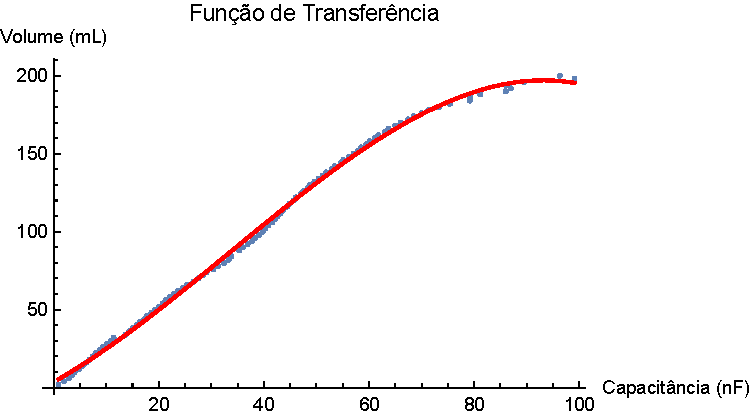
\includegraphics[width=\textwidth]{Nivel/TransferFunctionPlot.pdf}
	\caption{Função de Transferência experimental da capacitância do sensor}
	\label{fig:tf:nivel:capacitancia}
\end{figure}

Na Figura \ref{fig:tf:nivel:capacitancia} a linha contínua é um polinômio de terceira ordem regredido por mínimos quadrados conforme Equação \ref{eq:tf:nivel:capacitancia}

\begin{equation}
	V(C) = 3.585 + 1.896 C + 0.0261 C^2 - 0.000259 C^3
	\label{eq:tf:nivel:capacitancia}
\end{equation}
\noindent onde $V(C)$ é a função de volume de líquido (em mL) em função da capacitância medida no sensor ($C$).

A Equação \ref{eq:tf:nivel:capacitancia} foi ajustada com $R^2$ dado pela Equação \ref{eq:tf:nivel:capacitancia-r2} 

\begin{equation}
	R^2 = 0.999606
	\label{eq:tf:nivel:capacitancia-r2}
\end{equation}

Pela Figura \ref{fig:tf:nivel:capacitancia} é visivel que o sensor é linear até 180 mL, após ele passa a ter erros significativos na leitura.

Foi testado também o efeito da temperatura no valor de capacitância do sensor. Neste teste, o fundo de escala (200 mL) foi aquecido até 40ºC e a capacitância foi medida. Houve uma variação de 20 nF do valor esperado. Este teste prova a necessidade de compensação térmica do valor.

A proposta é que sejam colocados eletrodos de referência no fundo do recipiente e que o valor de capacitância deste sensor seja utilizado como referência do ponto zero do sistema, isto é, o ponto em que o volume é zero (1-2mm de coluna de água).


\begin{thebibliography}{9}
\bibitem{mathematica-numerial-precision} \url{https://reference.wolfram.com/language/tutorial/NumericalPrecision.html}, acessado em 16 de março de 2016

\bibitem{livro-texto}  Balbinot, A.; Brusamarello, V. J., Instrumentação e Fundamentos de Medida - Vol.1 - 2ª Ed. Rio de Janeiro: LTC, 2014.

\bibitem{estacao} \url{https://pt.wikipedia.org/wiki/Esta\%C3\%A7\%C3\%A3o_meteorol\%C3\%B3gica}, acessado em 16/04/2016.

\bibitem{pluviometro} \url{https://pt.wikipedia.org/wiki/Pluvi\%C3\%B4metro}, acessado em 16/04/2016.
\bibitem{pluviometro-1} \url{http://www.agsolve.com.br/dicas-e-solucoes/como-funciona-o-pluviometro}, acessado em 16/04/2016.

\bibitem{catalogo-pt100} Catálogo de sensores resistivos de platina da LABFACILITY, \url{http://www.farnell.com/datasheets/1848446.pdf }, acessado em 31/05/2016.

\bibitem{datasheet-INA126} Datasheet do amplificador de instrumentação INA126, da Texas Instruments, disponível em \url{http://www.ti.com.cn/cn/lit/ds/symlink/ina126.pdf}.

\bibitem{pluviometro-capacitivo-texas} Capacitive-Based Liquid Level Sensing Sensor Reference Design, \url{http://www.ti.com/lit/ug/tidu736a/tidu736a.pdf
}, acessado em 30/05/2016.

\bibitem{medicao-capacitancia} Use Analog Techniques To Measure Capacitance In Capacitive Sensors, \url{http://m.electronicdesign.com/analog/use-analog-techniques-measure-capacitance-capacitive-sensors}, acessado em 01/06/2016.

\bibitem{multimetro-minipa} Manual do multímetro digital Minipa ET-2082B, disponível em \url{http://portal.if.usp.br/labdid/sites/portal.if.usp.br.labdid/files/Et-2082b-1100.pdf}.


%\bibitem{ref1} Sobrenome, A.B.; Sobrenome, C.D. Title of the cited article. Journal Title 2007, 6, 100-110. 
%\bibitem{ref2} Balbinot, A.; Brusamarello, V.J.. Title of the cited article. Journal Title 2007, 6, 100-110. 
%\bibitem{ref3} Author, A.; Author, B. Title of the chapter. In Book Title, 2nd ed.; Editor, A., Editor, B., Eds.; Publisher: Publisher Location, Country, 2007; Volume 3, pp. 154-196.
%\bibitem{ref4} Author, A.; Author, B. Book Title, 3rd ed.; Publisher: Publisher Location, Country, 2008; 
%pp. 154-196.

\end{thebibliography}

\end{document}
